\section{Introduction}

\lettrine[lines=3]{I}{n number theory}, a perfect number is a
positive integer that is equal to the sum of its positive divisors,
excluding the number itself (called its \emph{proper divisors}). For instance, $6$ has divisors $1, 2$ and
$3$ (excluding itself), and $1 + 2 + 3 = 6$, so $6$ is a perfect number.

The sum of divisors of a number, excluding the number itself, is
called its \emph{aliquot sum}, $s (n)$ of a positive integer $n>0$
is the sum of all \emph{proper divisors} of $n$, that is, all
divisors of $n$ other than $n$ itself.  When we write $d\mid n$ we mean
that $n \div d$ is an integer with no remainder, and when we write
$d \nmid n$ then $n \div d$ has a remainder.  So we define $s(n)$ as,
$$s (n)=\sum\nolimits_{d\mid n,\ 0<d < n}d.$$
A perfect number is one that is equal to its aliquot sum. Equivalently, a perfect number
is a number that is half the sum of all of its positive divisors including itself; in symbols,
$\sigma_1 (n) = 2 n$ where $\sigma_1$
is the sum-of-divisors function.
That is,
$$\sigma_1 (n)=\sum\nolimits_{d\mid n,\ 0<d\le n}d.$$
For instance, $28$ is perfect as
$\sigma_1(28) = 1 + 2 + 4 + 7 + 14 + 28 = 56 = 2 \times 28$.
When you see the $\Sigma$ symbol (or the $\Pi$ symbol), you should think of a \texttt{for} loop.

In about 300\xspace BC, Euclid
showed that if $2^p - 1$
is prime then $2^{p-1}(2^p -1)$
is perfect.  The first four perfect numbers were the only ones known
to the early Greek mathematicians, and the mathematician \emph{Nicomachus}
noted that $8\,128$ was perfect as early as around AD\xspace 100.

In modern language, Nicomachus states without proof that \emph{every}
perfect number is of the form $2^{n-1}(2^n-1)$ where $2^n-1$ is
prime.  He says of perfect numbers, ``There is a method of producing
them, neat and unfailing, which neither passes by any of the perfect
numbers nor fails to differentiate any of those that are not such,
which is carried out in the following way.'' He then goes on to
explain a procedure which is equivalent to finding a \emph{triangular
number} based on a Mersenne prime.  He seems to be unaware that $n$
itself has to be prime. He also says (wrongly) that the perfect
numbers end in $6$ or $8$ alternately. (The first $5$ perfect numbers
end with digits $6$, $8, 6, 8$ and $6$; but the sixth also ends in
$6$.) It is important that you understand that not every number of
the form $2^{n-1}(2^n-1)$ is perfect, but every perfect number is
of the form $2^{n-1}(2^n-1)$.
Are there any odd perfect numbers? \emph{We do not know.}

\emph{Philo of Alexandria}
in his first-century book \emph{On the Creation} mentions perfect numbers,
claiming that the world was created in $6$ days and the moon orbits
in $28$ days because $6$ and $28$ are perfect. Philo is followed by
\emph{Origen}
and by \emph{Didymus the Blind},  who adds the
observation that there are only four perfect numbers that are less
than $10\,000$.
Saint Augustine defines perfect
numbers in \emph{City of God} (Book XI, Chapter 30)
in the early $5^\text{th}$ century AD, repeating the claim that God created
the world in $6$ days because $6$ is the smallest perfect number.
The
Egyptian mathematician Ismail ibn Fall\={u}s (1194--1252) mentioned the
next three perfect numbers ($33\,550\,336$; $8\,589\,869\,056$ and
$137\,438\,691\,328$) and listed a few more which are now known to be
incorrect.

The first known European
mention of the fifth perfect number is a manuscript written between
1456 and 1461 by an unknown mathematician.
In 1588, the Italian mathematician \emph{Pietro Cataldi} identified
the sixth ($8\,589\,869\,056$) and the seventh ($137\,438\,691\,328$) perfect
numbers, and also proved that every perfect number obtained from
Euclid's rule ends with a $6$ or an $8$.

You should know that a \emph{prime number} is one that is only divisible by itself and $1$, or for $n>2$ ($n$ is the first prime), for $2\le x < n, x \nmid n$. Finding primes can be tedious, but in this assignment we will be looking at all proper divisors so using \emph{trial division} is appropriate.

In summary, a \emph{perfect number} $n$ is one where $s(n) = n$,
and a \emph{deficient number} is one where $s(n) < n$ and an
\emph{abundant number} is one where $s(n) > n$.

% \begin{center}
% \fbox{\begin{minipage}{0.85\textwidth}
% \emph{Question:} Do you really need to try \emph{all} $x < n$, or can you stop sooner? If so, when can you safely stop?
% \end{minipage}}
% \end{center}

\begin{figure}
        \centering
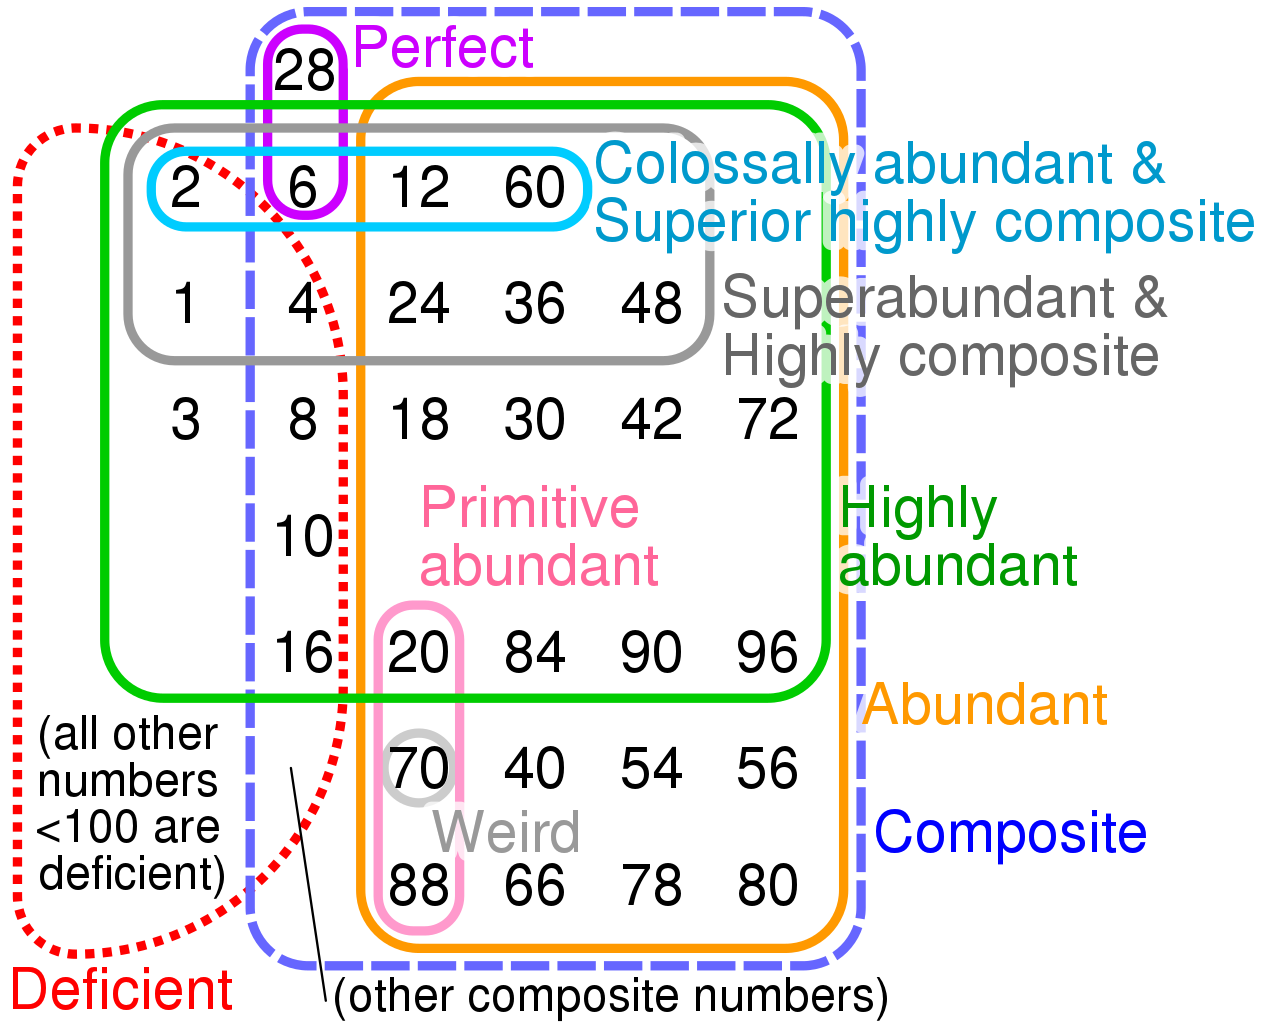
\includegraphics[width=0.5\textwidth]{images/euler-diagram.png}
        \caption{Euler Diagram of $1, \ldots, 100$}\label{fig:euler}
\end{figure}

\begin{center}
\fbox{\begin{minipage}{0.9\textwidth}
If you look carefully at Figure\xspace\ref{fig:euler}, you might understand why measurement systems other than \emph{metric} are as they are. Why does the day have 24 hours? The hour 60 minutes? Why are there 360$^\circ$ in a circle? Why does the foot have 12 inches? The yard 36 inches? Humans find
fractions easier than repeating decimals.
\end{minipage}}
\end{center}
